
\documentclass{configs/idp-model}
\usepackage{float}
\usepackage{xurl}
\usepackage{algorithm}
\usepackage{algpseudocode}


\usepackage{pgfplots}
\pgfplotsset{compat=1.17}

\usepackage{graphicx}
\graphicspath{{./figuras/}{./}}

\usepackage{booktabs}
\usepackage{array}

\autor{Matheus Antônio de Castro de Barros}
\engenhariadesoftware
\titulo{Acceleration of Pattern Matching Algorithms Using Parallel Programming}
\ano{2026}
\orientador{Jeremias Moreira Gomes}

\palavraschave{Aho--Corasick, Programação Paralela, Casamento de Múltiplos Padrões, POSIX Threads, Detecção de Intrusão}
\keywords{
  Aho–Corasick,
  parallel programming,
  parallel computing,
  multi-pattern matching,
  POSIX threads%
}

\dataaprovacao{08/07/2026}



\begin{document}

\pagenumbering{roman}
\capaprincipal
\folharosto
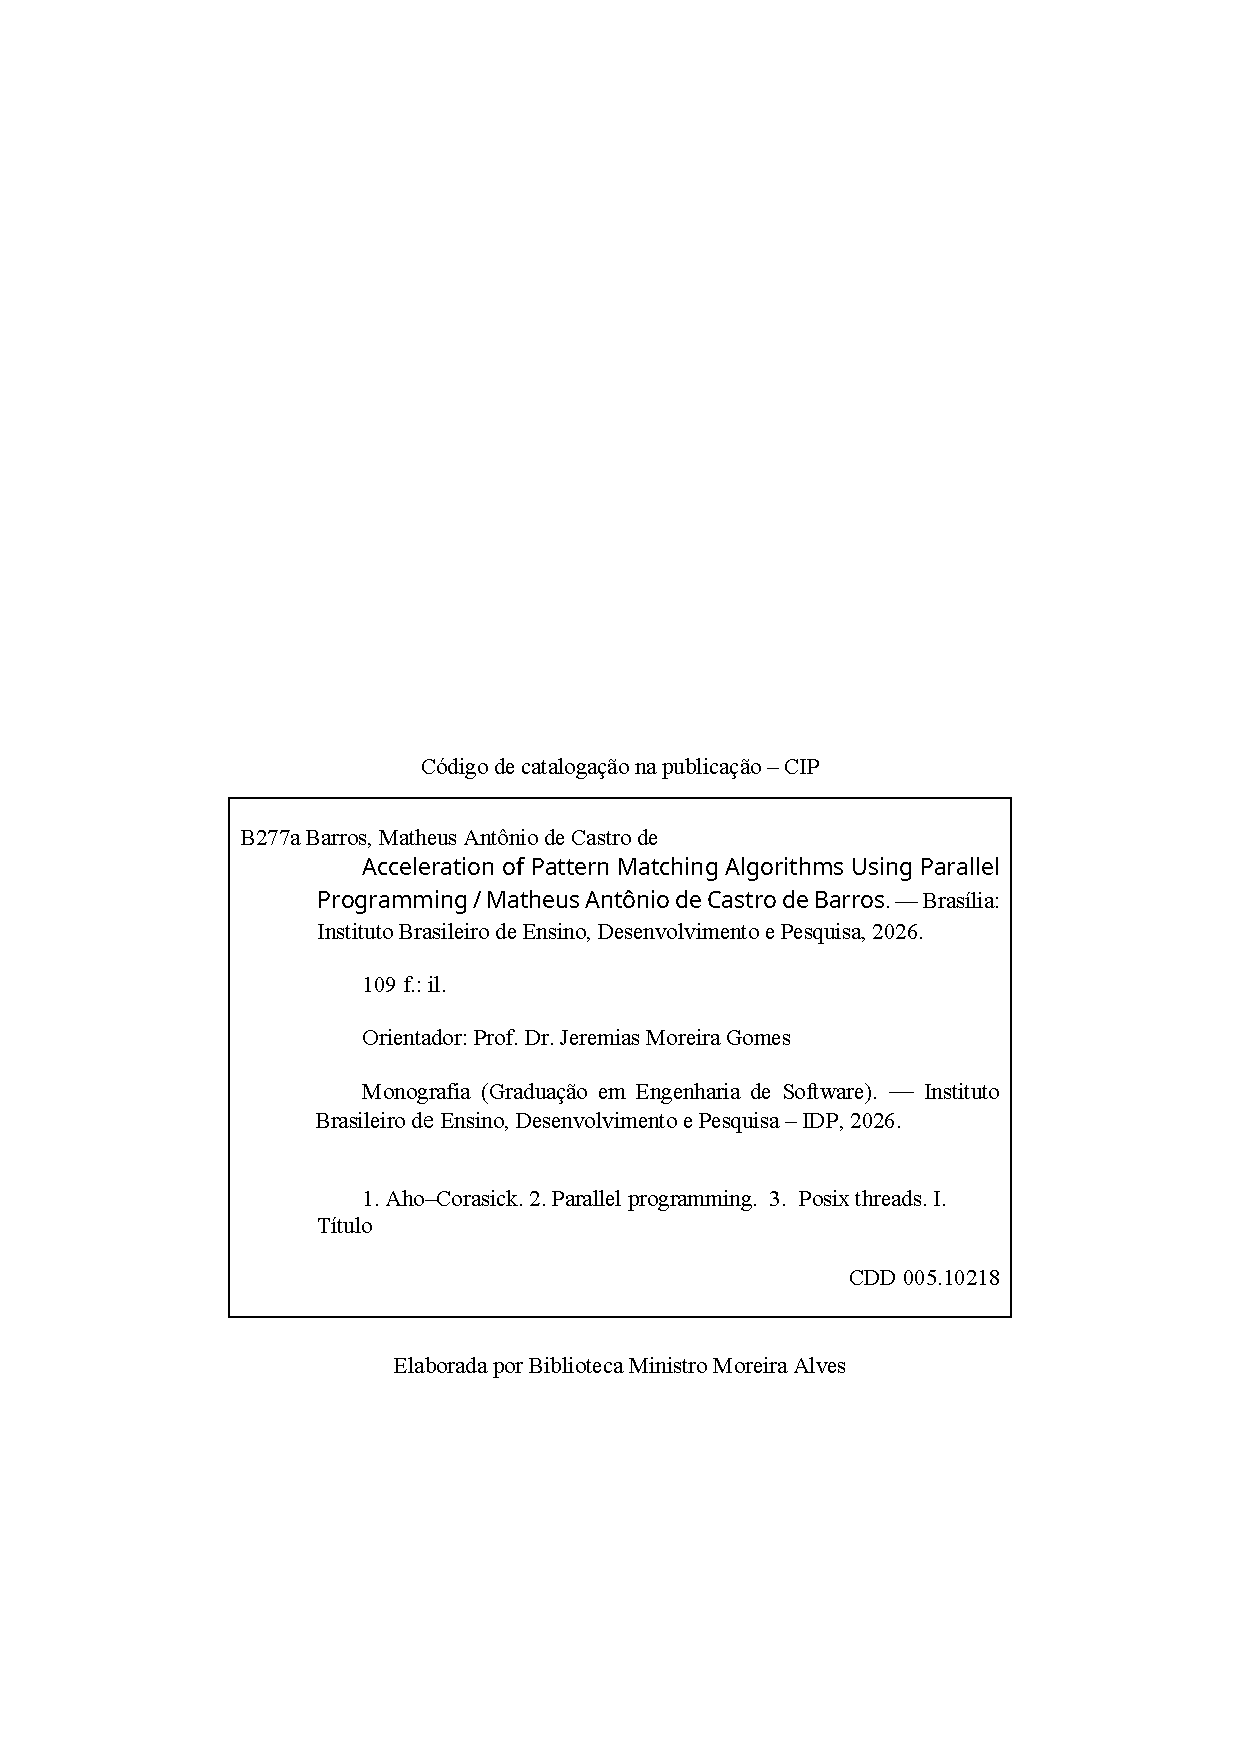
\includepdf{figuras/ficha-catalografica.pdf}
\folhaaprovacao

\dedicatoria
\agradecimentos

\abstract
\resumo

\listoffigures
\listoftables

\tableofcontents
\pagenumbering{arabic}

\secao{Introduction}{partes/introduction}
\secao{Theoretical Framework}{partes/fundamentacao}
\secao{Systematic Review}{partes/rsl}
\secao{Proposed Solution}{partes/proposal}
\secao{Methodology}{partes/methodology}
\secao{Results and Discussion}{partes/results}
\secao{Conclusion}{partes/conclusion}

\referencias

\apendice{Database Query Protocol}{partes/apendicei}

\capafinal

\end{document}
